\appendix

\chapter{Properties of Pauli Matrices}
\label{app:pauli_properties}

The Pauli matrices are essential building blocks in quantum mechanics and quantum computing. They are given in Definition~\ref{def:pauli_matrices}
\section{Commutation Relations}
\label{appsec:commutation_relations}

The commutation relation for the Pauli matrices $ \sigma_x, \sigma_y$ and $ \sigma_z$ is given by
\begin{align}
  \label{eq:pauli_commutation_relation}
  \left[ \sigma_i, \sigma_j \right] = 2 i \epsilon_{ijk} \sigma_k,
\end{align}
where $ \epsilon_{ijk}$ is the Levi-Civita symbol. 

The anticommutation relation for the \textbf{fermionic} creation and annihilation operators $ a_i$ and $ a_i^\dagger$ is given by
\begin{align}
  \label{eq:creation_annihilation_commutation_relation}
  \left\{ a_i, a_j \right\} = \left\{ a_i^\dagger, a_j^\dagger \right\} = 0, \quad \left\{ a_i, a_j^\dagger \right\} = \delta_{ij}.
\end{align}

\section{Pauli Matrices as Basis}
\label{appsec:pauli_basis}
The Pauli matrices $ \sigma_x, \sigma_y $ and $ \sigma_z $ form a basis for the space of $ 2 \times 2$ matrices. Any matrix $M$,
\[ M = \begin{pmatrix} 
\alpha & \beta \\ \gamma & \delta \
\end{pmatrix}. \] 
can be written as a linear combination of the Pauli matrices,
\[ M = \left( a \mathbb{I} + b \sigma_x + c \sigma_y + d \sigma_z \right), \]
\[ a 
	\begin{pmatrix} 1 & 0 \\ 0 & 1 \end{pmatrix} + b \begin{pmatrix} 0 & 1 \\1 & 0 \end{pmatrix} + c \begin{pmatrix} 0 & -i \\ i & 0 \end{pmatrix} + d \begin{pmatrix} 1 & 0 \\ 0 & -1 \end{pmatrix}.  \] 

the coefficients $a, b, c$ and $d$ can be found by solving the linear equations:
\begin{align}
	\label{eq:linear_eq_pauli}
	\alpha &= a + d, \\
	\beta &= b - i c, \\
	\gamma &= b + i c, \\
	\delta &= a - d.
\end{align}
Solving Equations~\eqref{eq:linear_eq_pauli} for $ a,b,c $ and $ d $ gives
\begin{align}
	\label{eq:solve_linear_eq_pauli}
	a &= \frac{1}{2} \left( \alpha + \delta \right) = \frac{1}{2} \tr{IM}, \\
	b &= \frac{1}{2} \left( \beta + \gamma \right) = \frac{1}{2}\tr{XM}, \\
	c &= \frac{1}{2i} \left( \gamma - \beta \right) = \frac{1}{2} \tr{YM}, \\
	d &= \frac{1}{2} \left( \alpha - \delta \right) = \frac{1}{2}\tr{ZM}. \\
\end{align}
In fact, this generalises. For a new matrix $ A $ of size $ 2^n \times 2^n $, given that $ \{ P_i \} $ is a set of orthonormal basis of the dimension. Then $ A $ can be written as a linear combination of the basis $ \{ P_i \} $,
\[ A = \sum_{j}a_jP_j. \]
Products of Pauli matrices is given in Table~\ref{tab:pauli_prod}. It is not hard to see that the trace of these products can be expressed as 
\[ \tr{\sigma_j\sigma_k} = 2^n \delta_{jk},\] since the Pauli matrices are traceless. The $ 2^n $ term comes from the trace of the identity matrix in $ 2^n $ dimension.
For an arbitrary coefficient $ a_k $ corresponding to the basis $ B_k $, following the above equation we have
\begin{align*}
	\label{eq:proof-of-pd}
	P^{\dagger}_kA  &= P_k^{\dagger}\sum_{j} a_j P_j, \\
	P^{\dagger}_k A &= \sum_j a_j \tr{P_k^{\dagger}P_j}, \quad\quad \text{Linearity of summation}\\
	\tr{P^{\dagger}_k A} &= \sum_j a_j \tr{P_k^{\dagger}P_j}, \quad\quad \text{Linearity of trace} \\
	\tr{P^{\dagger}_k A} &= \sum_j  2^n a_j\delta_{jk},   \\
	a_k &= \frac{1}{2^n}\tr{P^{\dagger}_k A}.
\end{align*}
Tensor products of Pauli matrices form a basis for the space of $ 2^n \times 2^n$ matrices due to the linearity of the tensor product. This proves Equation~\eqref{eq:pauli-decomp}.

\section{Product of Pauli Matrices}
Table~\ref{tab:pauli_prod} shows the matrix products of pairs of Pauli matrices.
\begin{table}[ht]
	\centering
	\caption{Products of two Pauli matrices (Row $\times$ column).}
	\label{tab:pauli_prod}

	\begin{tabular}{c c c c}
		\toprule
		 & $ \sigma_x $ & $ \sigma_y $ & $ \sigma_z $ \\
		\midrule
		$\sigma_x $ & $I$ & $i \sigma_z$ & $ -i \sigma_y$ \\
		$\sigma_y$ & $ -i \sigma_z$ & $ I $ & $ i \sigma_x$ \\
		$ \sigma_z$ & $ i \sigma_y$ & $ -i \sigma_x$ & $ I $ \\
		\bottomrule
	\end{tabular}
\end{table}

\chapter{The Vanishing ADAPT gradient}
\label{app:zerograd}

In this appendix we will show that the operator gradient given by Equation~\eqref{eq:A-gradient} for the $ 3 $-qubit qubit-ADAPT pool is $ 0 $ for the $ \ket{0} $ state using the example Hamiltonian given in Equation~\eqref{eq:0gradHamiltonian}. 

We showed in Section~\ref{sec:initstate} that the gradient of the state $ \ket{0\ldots0} $ is $ 0 $ for one of the operators, $ iYZZ $. We will show that this is true for the other three operators in the pool, given in Equation~\eqref{eq:matrixiIYZ}, \eqref{eq:matrixiIIY}, \eqref{eq:matrixiIYI}.

\begin{equation}
	\label{eq:matrixiIYZ}
	iIYZ = \begin{pmatrix} 
	0 & 0 & 1 & 0 & 0 & 0 & 0 & 0 & \\ 
	0 & 0 & 0 & -1 & 0 & 0 & 0 & 0 & \\ 
	-1 & 0 & 0 & 0 & 0 & 0 & 0 & 0 & \\ 
	0 & 1 & 0 & 0 & 0 & 0 & 0 & 0 & \\ 
	0 & 0 & 0 & 0 & 0 & 0 & 1 & 0 & \\ 
	0 & 0 & 0 & 0 & 0 & 0 & 0 & -1 & \\ 
	0 & 0 & 0 & 0 & -1 & 0 & 0 & 0 & \\ 
	0 & 0 & 0 & 0 & 0 & 1 & 0 & 0 & \\   
\end{pmatrix},
\end{equation}

\begin{equation}
	\label{eq:matrixiIIY}
	iIIY = \begin{pmatrix} 
	0 & 1 & 0 & 0 & 0 & 0 & 0 & 0 & \\ 
	-1 & 0 & 0 & 0 & 0 & 0 & 0 & 0 & \\ 
	0 & 0 & 0 & 1 & 0 & 0 & 0 & 0 & \\ 
	0 & 0 & -1 & 0 & 0 & 0 & 0 & 0 & \\ 
	0 & 0 & 0 & 0 & 0 & 1 & 0 & 0 & \\ 
	0 & 0 & 0 & 0 & -1 & 0 & 0 & 0 & \\ 
	0 & 0 & 0 & 0 & 0 & 0 & 0 & 1 & \\ 
	0 & 0 & 0 & 0 & 0 & 0 & -1 & 0 & \\
\end{pmatrix},
\end{equation}

\begin{equation}
	\label{eq:matrixiIYI}
	iIYI = \begin{pmatrix}   
	0 & 0 & 1 & 0 & 0 & 0 & 0 & 0 & \\
	0 & 0 & 0 & 1 & 0 & 0 & 0 & 0 & \\
	-1 & 0 & 0 & 0 & 0 & 0 & 0 & 0 & \\
	0 & -1 & 0 & 0 & 0 & 0 & 0 & 0 & \\
	0 & 0 & 0 & 0 & 0 & 0 & 1 & 0 & \\
	0 & 0 & 0 & 0 & 0 & 0 & 0 & 1 & \\
	0 & 0 & 0 & 0 & -1 & 0 & 0 & 0 & \\
	0 & 0 & 0 & 0 & 0 & -1 & 0 & 0 & \\
	\end{pmatrix}.
\end{equation}

The following code snippet is the code used to numerically calculate the gradient for each operator with the same Hamiltonian, \[ \braket{\psi|[H,A]|\psi}.  \] 
\begin{mycode}
from Quanthon import pauli_sum, QubitAdaptAnsatz
from Quanthon.utils import get_pauli

def comm(A,B):
    if type(A) == str:
	A = get_pauli(A)
    if type(B) == str:
	B = get_pauli(B)
    
    return A@B - B@A
def grad(A, h_mat, state):
    return state.conj().T @ comm(h_mat, get_pauli(A)) @ state

qh = [('IIZ', 2), ('IXX', -0.5), ('IYY', 0.5), ('ZZI', 2)]
H = pauli_sum(qh)

qa = QubitAdaptAnsatz(3)
pool = qa.pool

for A in pool:
    A = A.strip('i')
    print(grad(A, H, Qubits(3).state))
\end{mycode}

The output of the code is as follows:
\begin{verbatim}
0j
0j
0j
0j
\end{verbatim}

This is a curious phenomenon as I have not seen it in relevant literature. To investigate this further, we will construct a 3-qubit Hamiltonian randomly while making sure every term possible exist. The code snippet is shown below. Since the pool is complete for all real states, we will also ignore terms with odd number of $ Y $ operators as they will not appear in a real Hamiltonian. The function \texttt{generate\_hermitian\_matrix} generate a random Hermitian matrix and \texttt{has\_odd\_y} is defined to g check if a given Pauli string has an odd number of $ Y $ operators.
\begin{mycode}
import numpy as np

n = 3
random_h = generate_hermitian_matrix(2**n)
all_ops = pauli_decomposition(random_h)
pool = QubitAdaptAnsatz(n).pool

# the zero state
state = np.zeros(2**n)
state[0] = 1

grad_zero_terms = []
real_terms = len(all_ops)

for term, coeff in all_ops:
	h_mat = get_pauli(term)
	
	if has_odd_y(term):
		real_terms -= 1
		continue
	zeros_count = 0
	for A in pool:
		
	    g = grad(A, h_mat, state)
	    if g == 0:
		    zeros_count += 1
	    if zeros_count == len(pool):
		    grad_zero_terms.append(term)

# print(grad_zero_terms)
print(f'{len(grad_zero_terms)} out of {real_terms} terms have zero gradient for all operators of the pool.')
\end{mycode}

The output of the code is as follows:
\begin{verbatim}
24 out of 36 terms have zero gradient for all operators of the pool.
\end{verbatim}
For $ n=4 $, 
\begin{verbatim}
104 out of 136 terms have zero gradient for all operators of the pool.
\end{verbatim}
This means initialising the state to $ \ket{0\ldots0} $ will result in a zero gradient for a significant number of terms in the Hamiltonian, causes the ADAPT-VQE to immidiately discard stop without converging to the actual ground state. We observed that by initialising the state randomly, while still keeping it real, the gradient is non-zero for all terms, except trivially the \texttt{I\ldots I} term.
\begin{mycode}
state = np.random.rand(2**n)
\end{mycode}
However, during the simulation we observed that this initialisation can lead to a poor convergence of the ADAPT-VQE. Another initial state \(\ket{+^{\otimes n}}\) has $ 58 $ out of the $ 136 $ terms with $ 0 $ gradient instead, but the convergence is much better than the random initialisation. 

\chapter{More Results}

\begin{figure}[h]
	\centering
	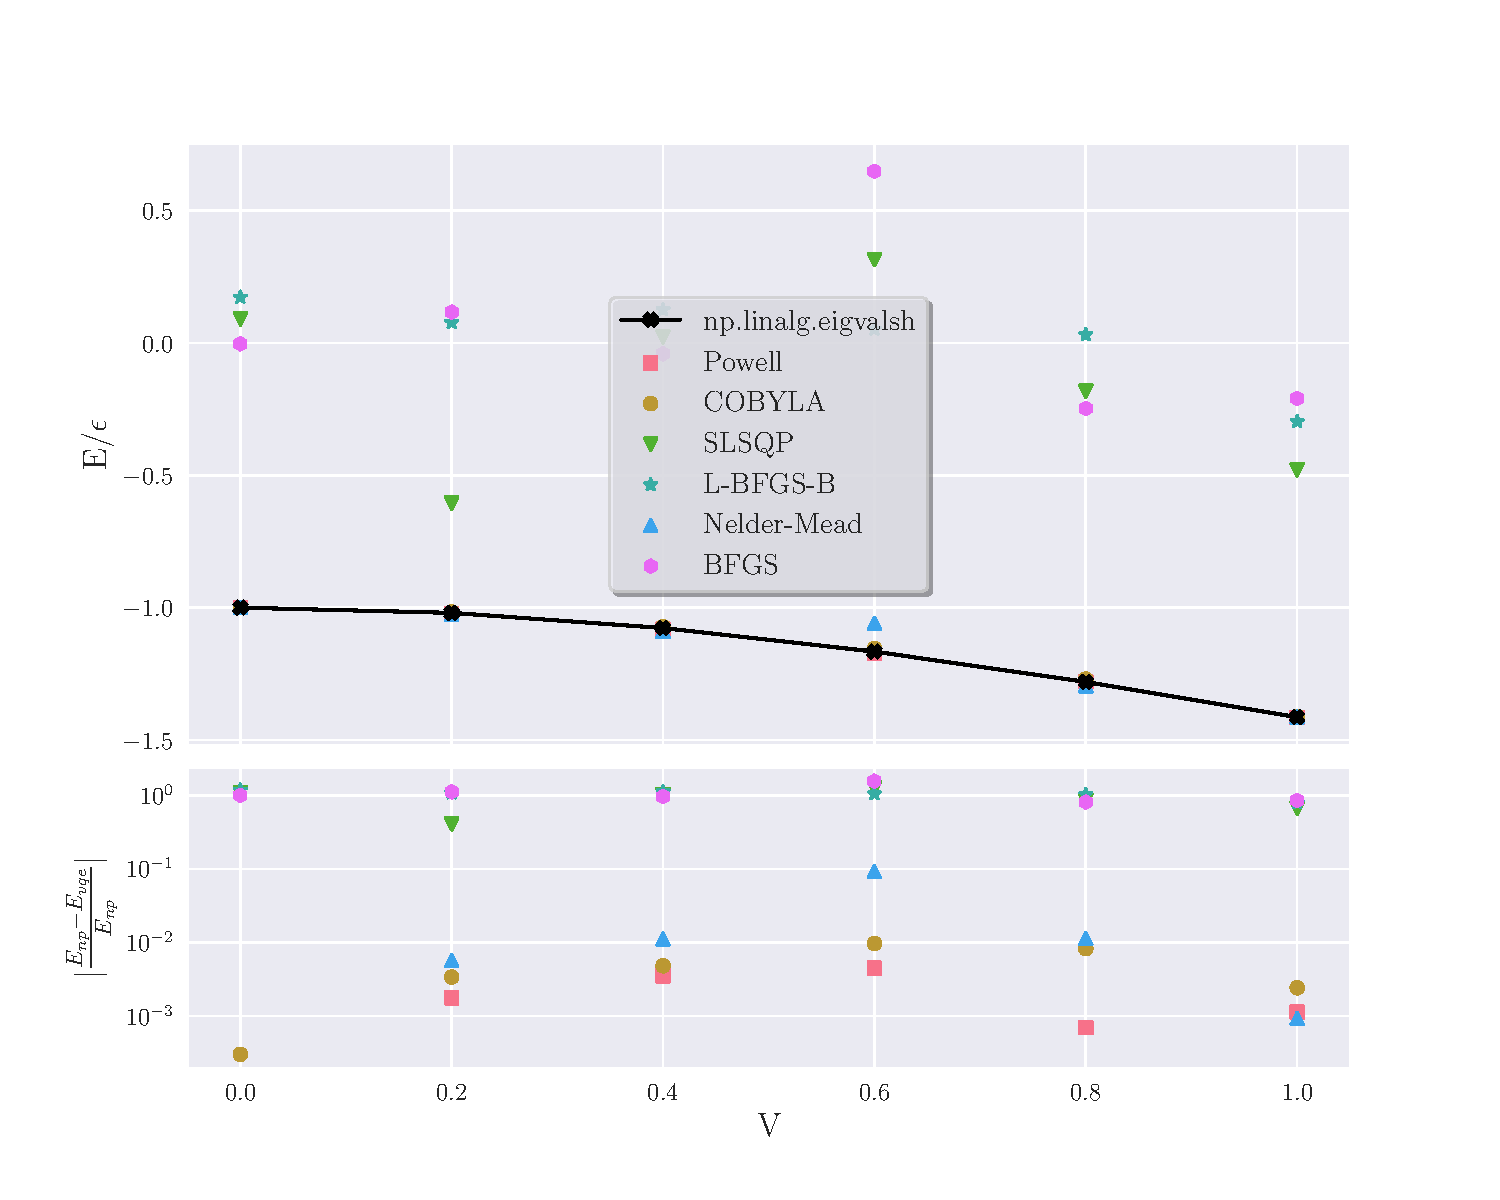
\includegraphics[width=0.32\linewidth]{image/lipkin_result/vqe-opt/cmp_opt_vqe_ee1000_J=1.pdf}
	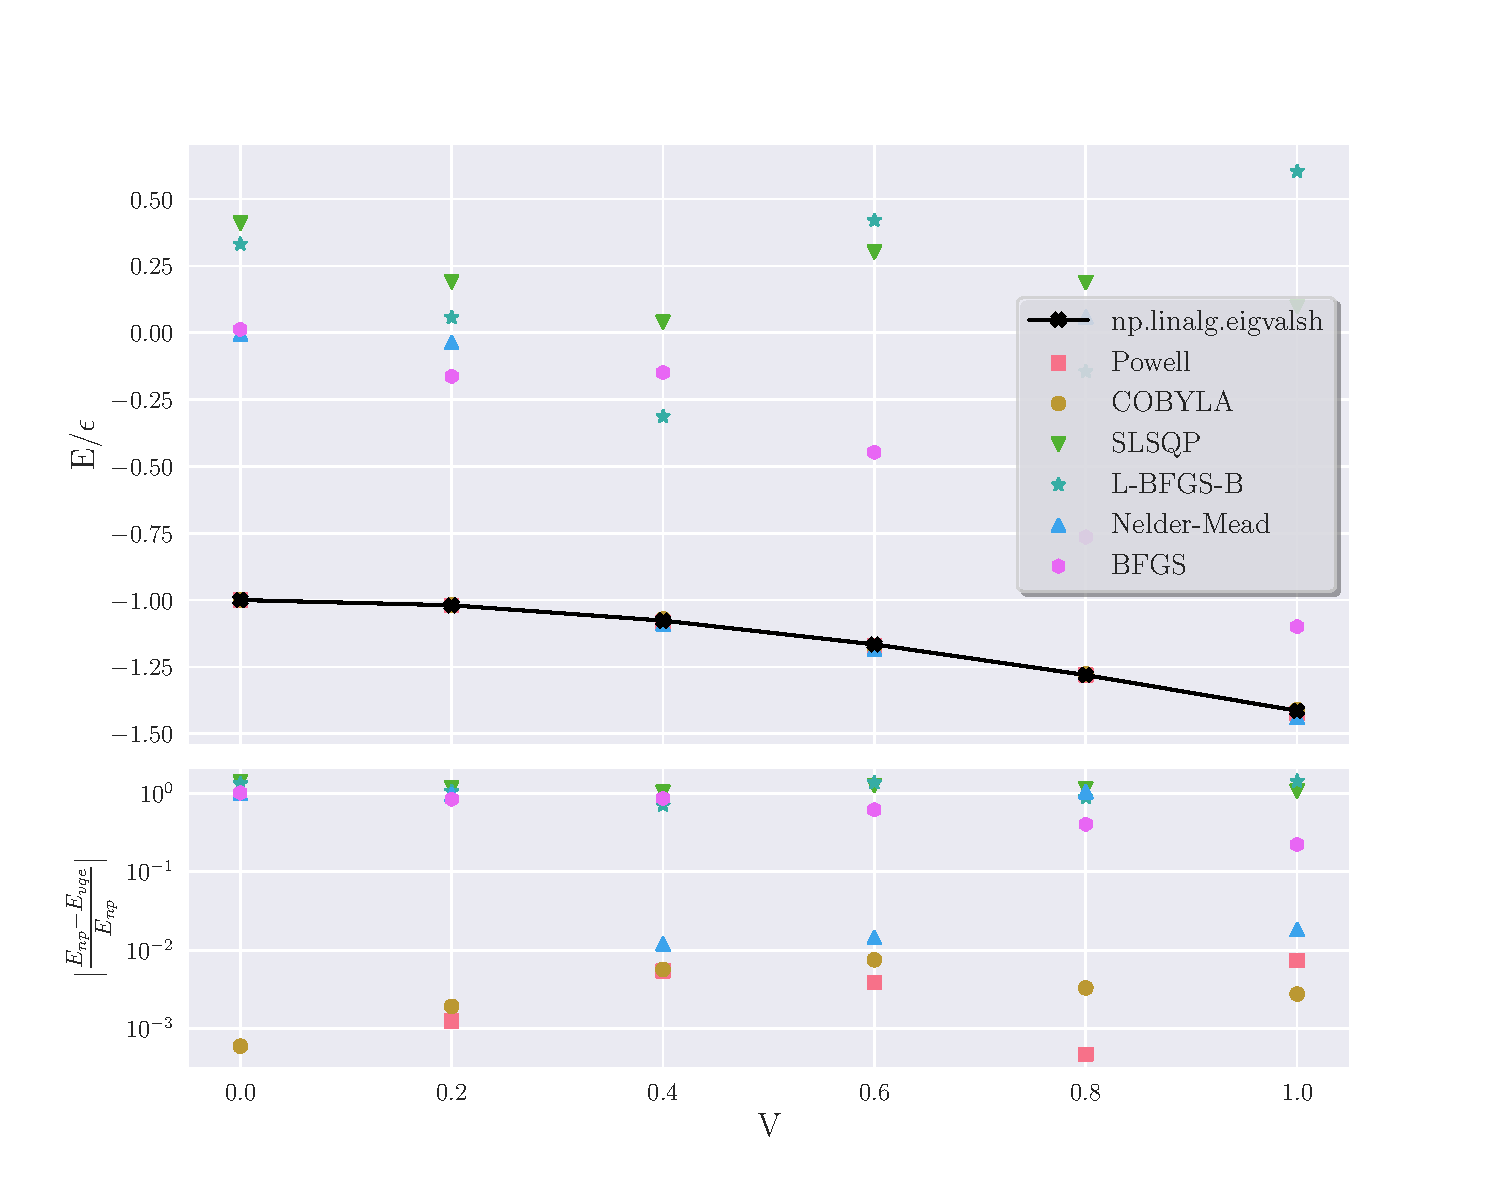
\includegraphics[width=0.32\linewidth]{image/lipkin_result/vqe-opt/cmp_opt_vqe_ee10000_J=1.pdf}
	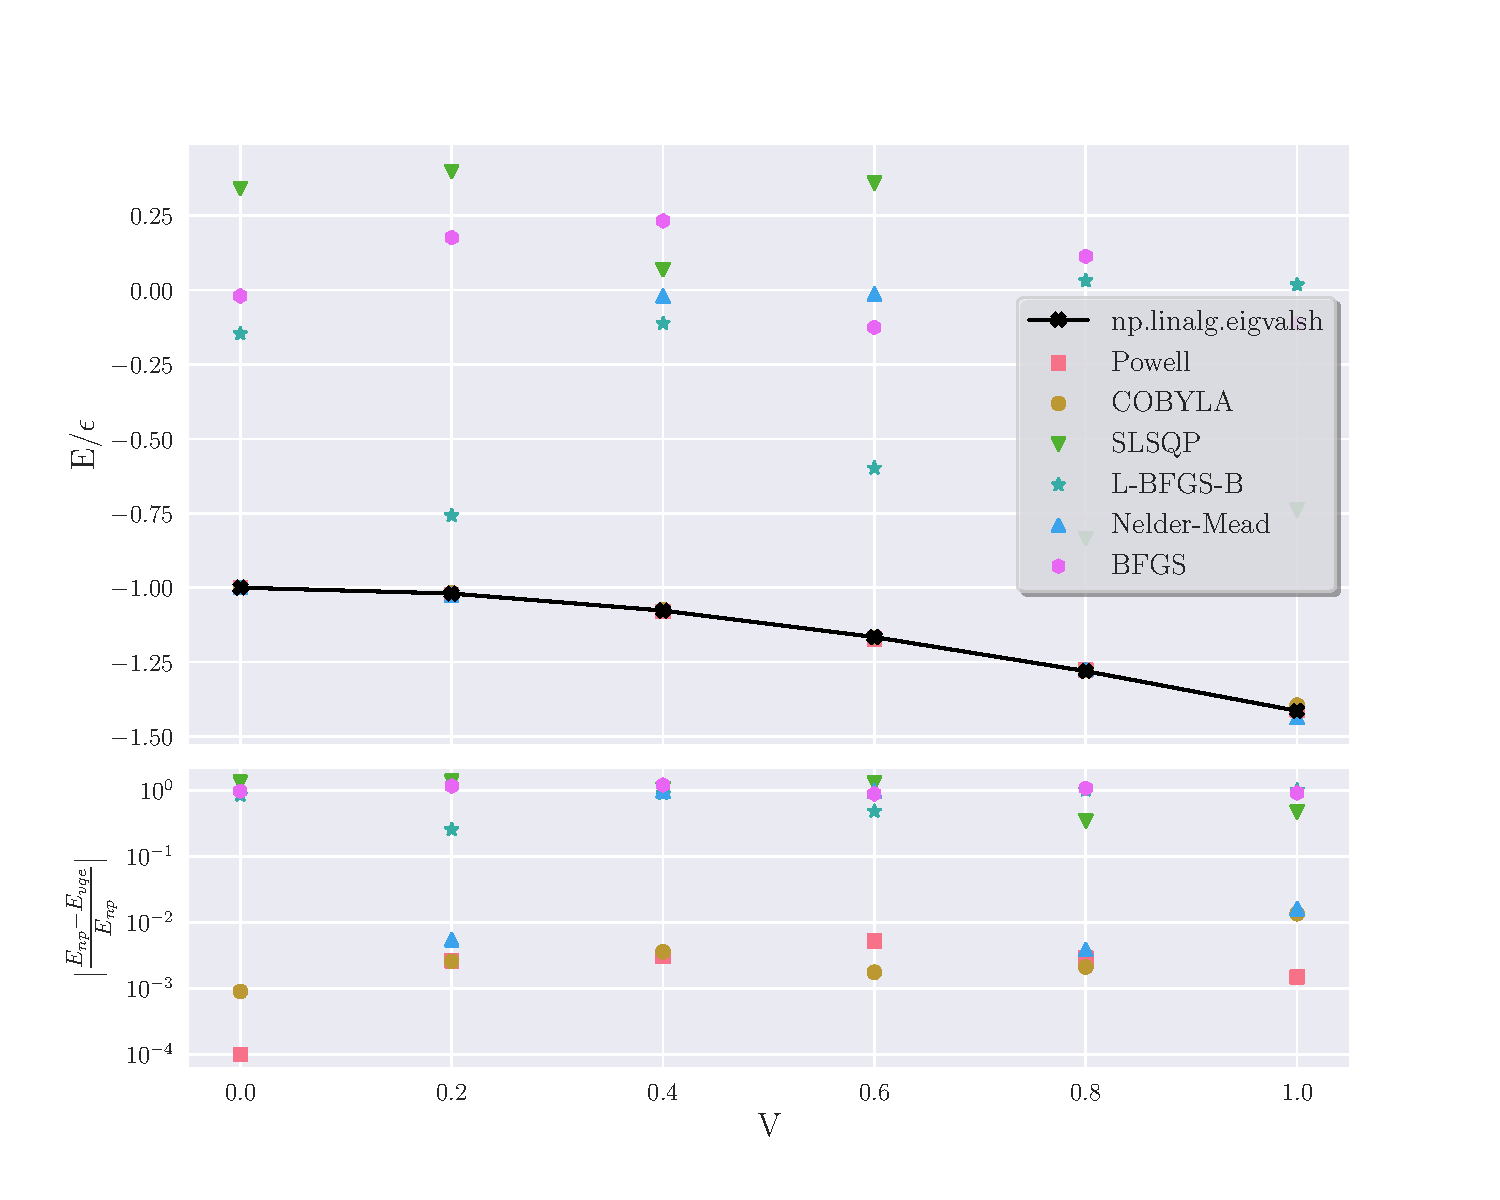
\includegraphics[width=0.32\linewidth]{image/lipkin_result/vqe-opt/cmp_opt_vqe_ee100000_J=1.pdf}
	\caption{Comparison amongst different optimisers for the fixed-form ansatz with \textbf{ieal simulation} for $ J=1 $. Different number of shots were used across all three figures: (left) $ 1000 $, (middle) $ 10000 $ and (right) $ 100000 $.}
	\label{fig:OptHW1}
\end{figure}

\begin{figure}[h]
	\centering
	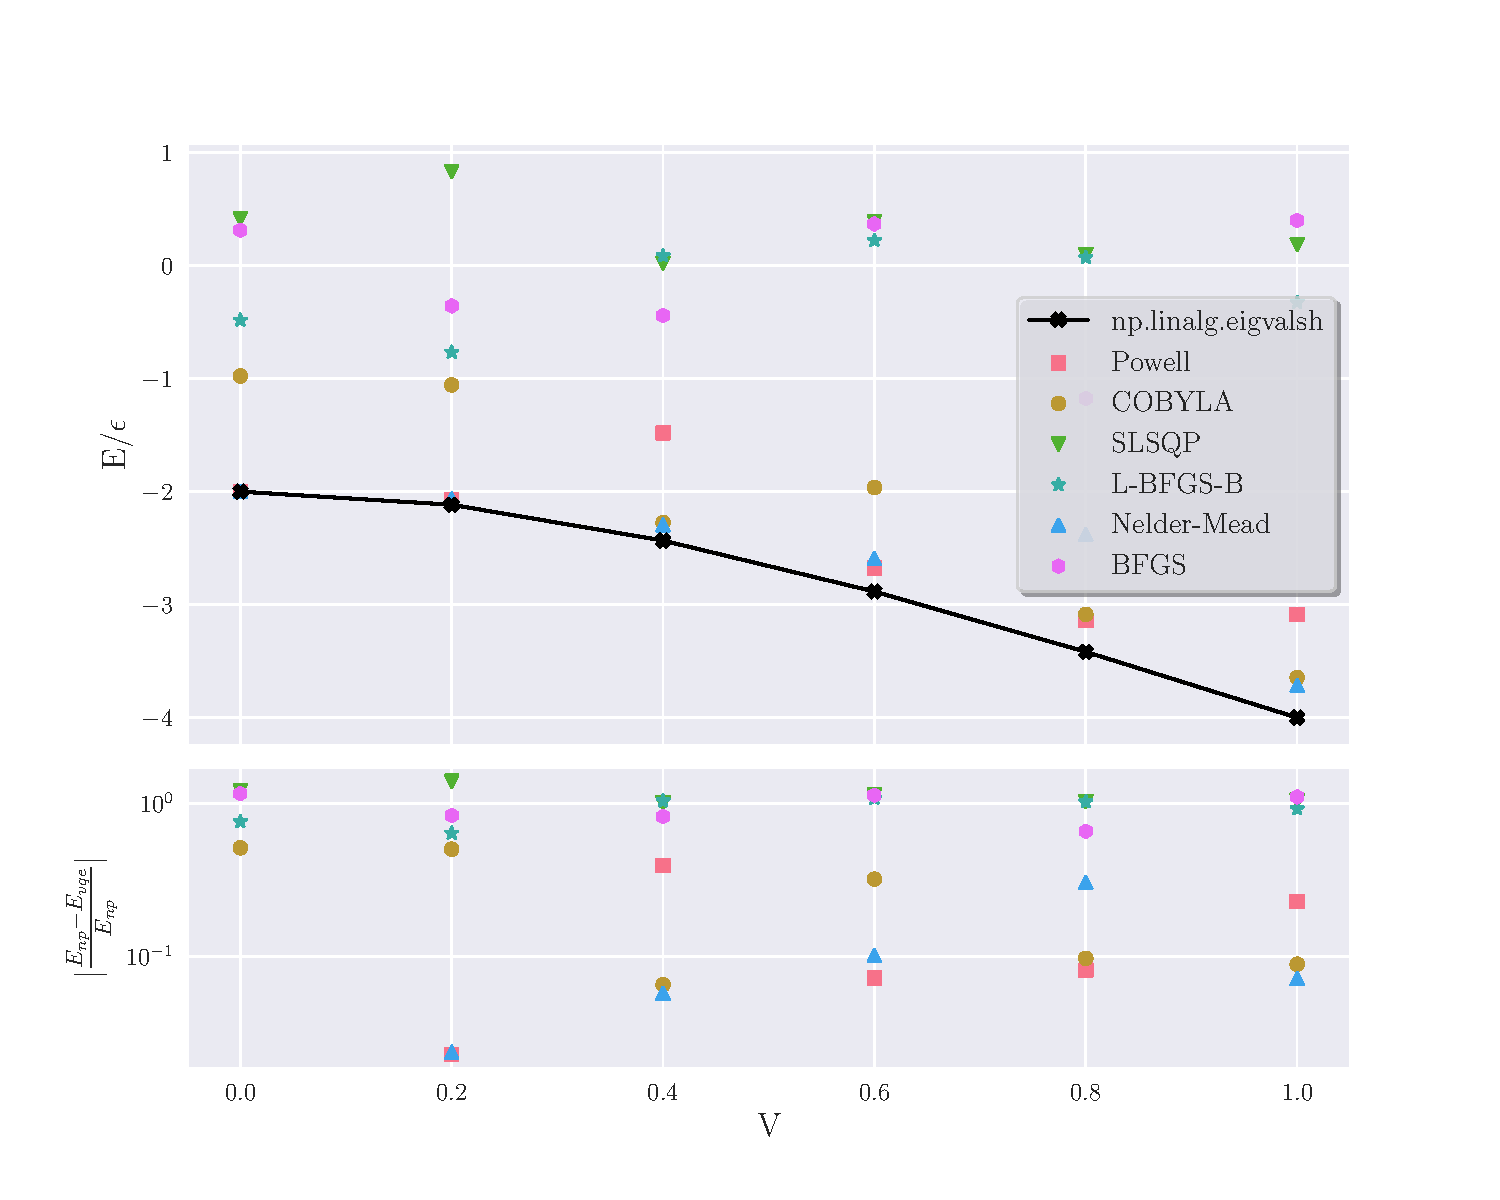
\includegraphics[width=0.32\linewidth]{image/lipkin_result/vqe-opt/cmp_opt_vqe_ee1000_J=2.pdf}
	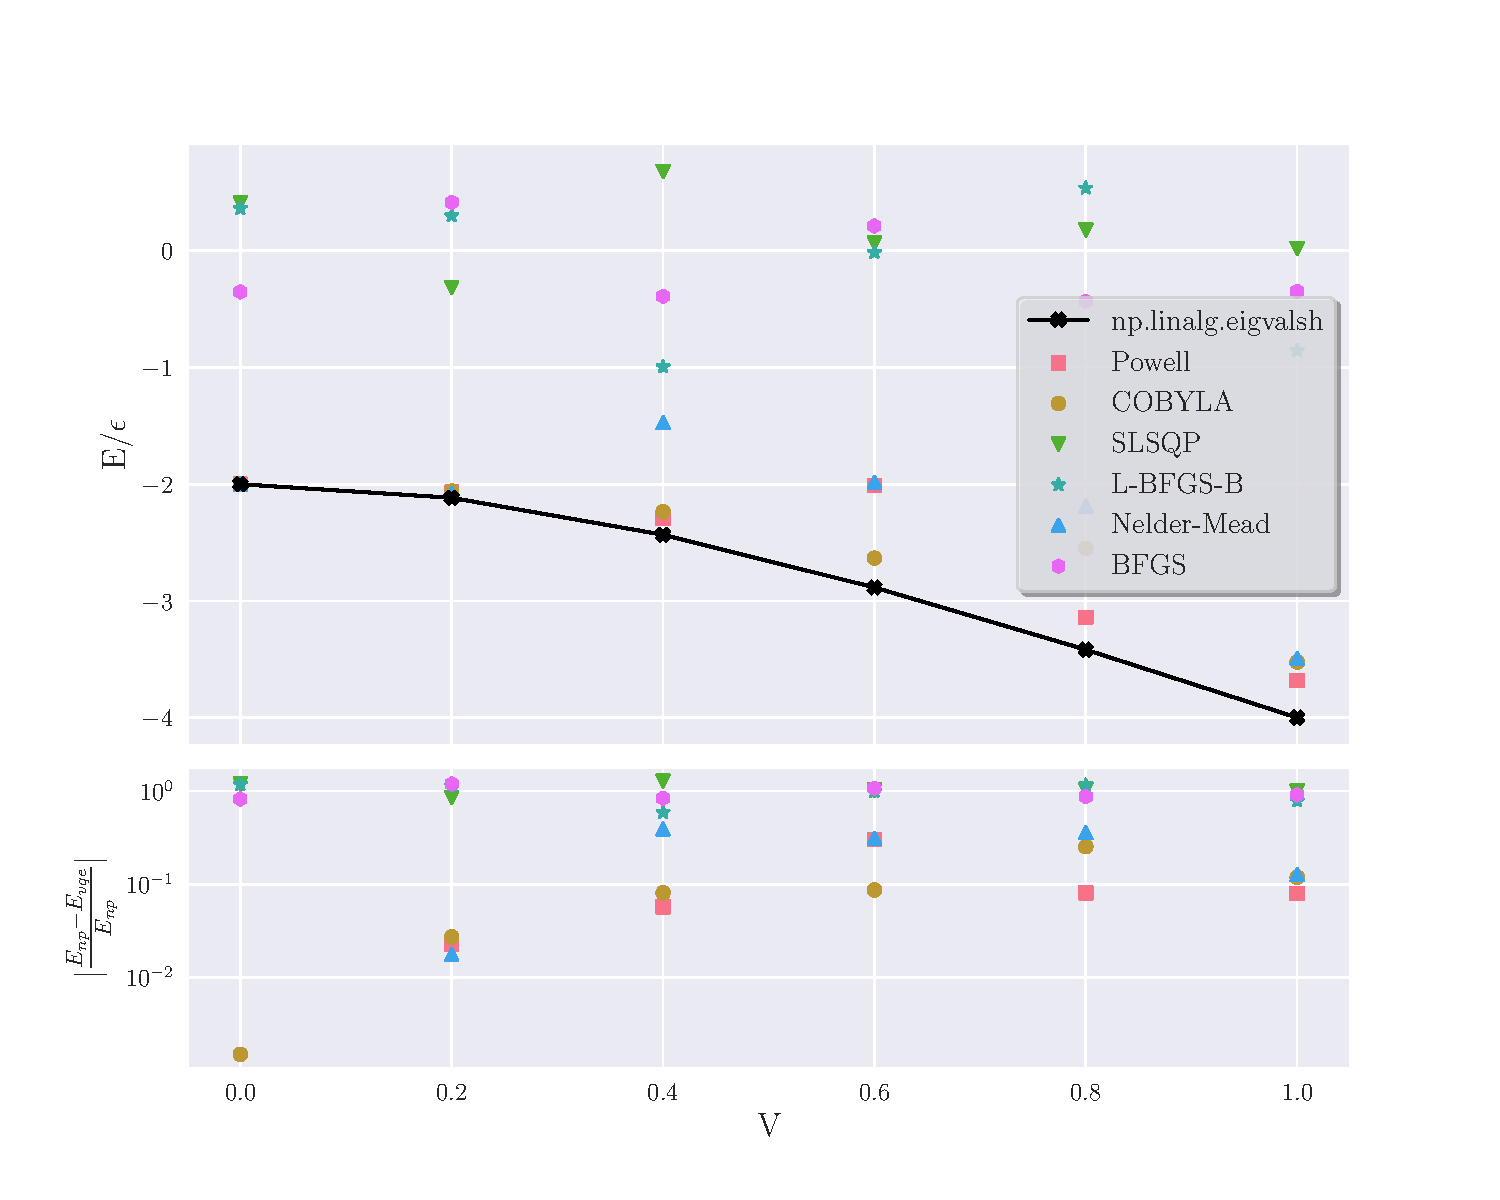
\includegraphics[width=0.32\linewidth]{image/lipkin_result/vqe-opt/cmp_opt_vqe_ee10000_J=2.pdf}
	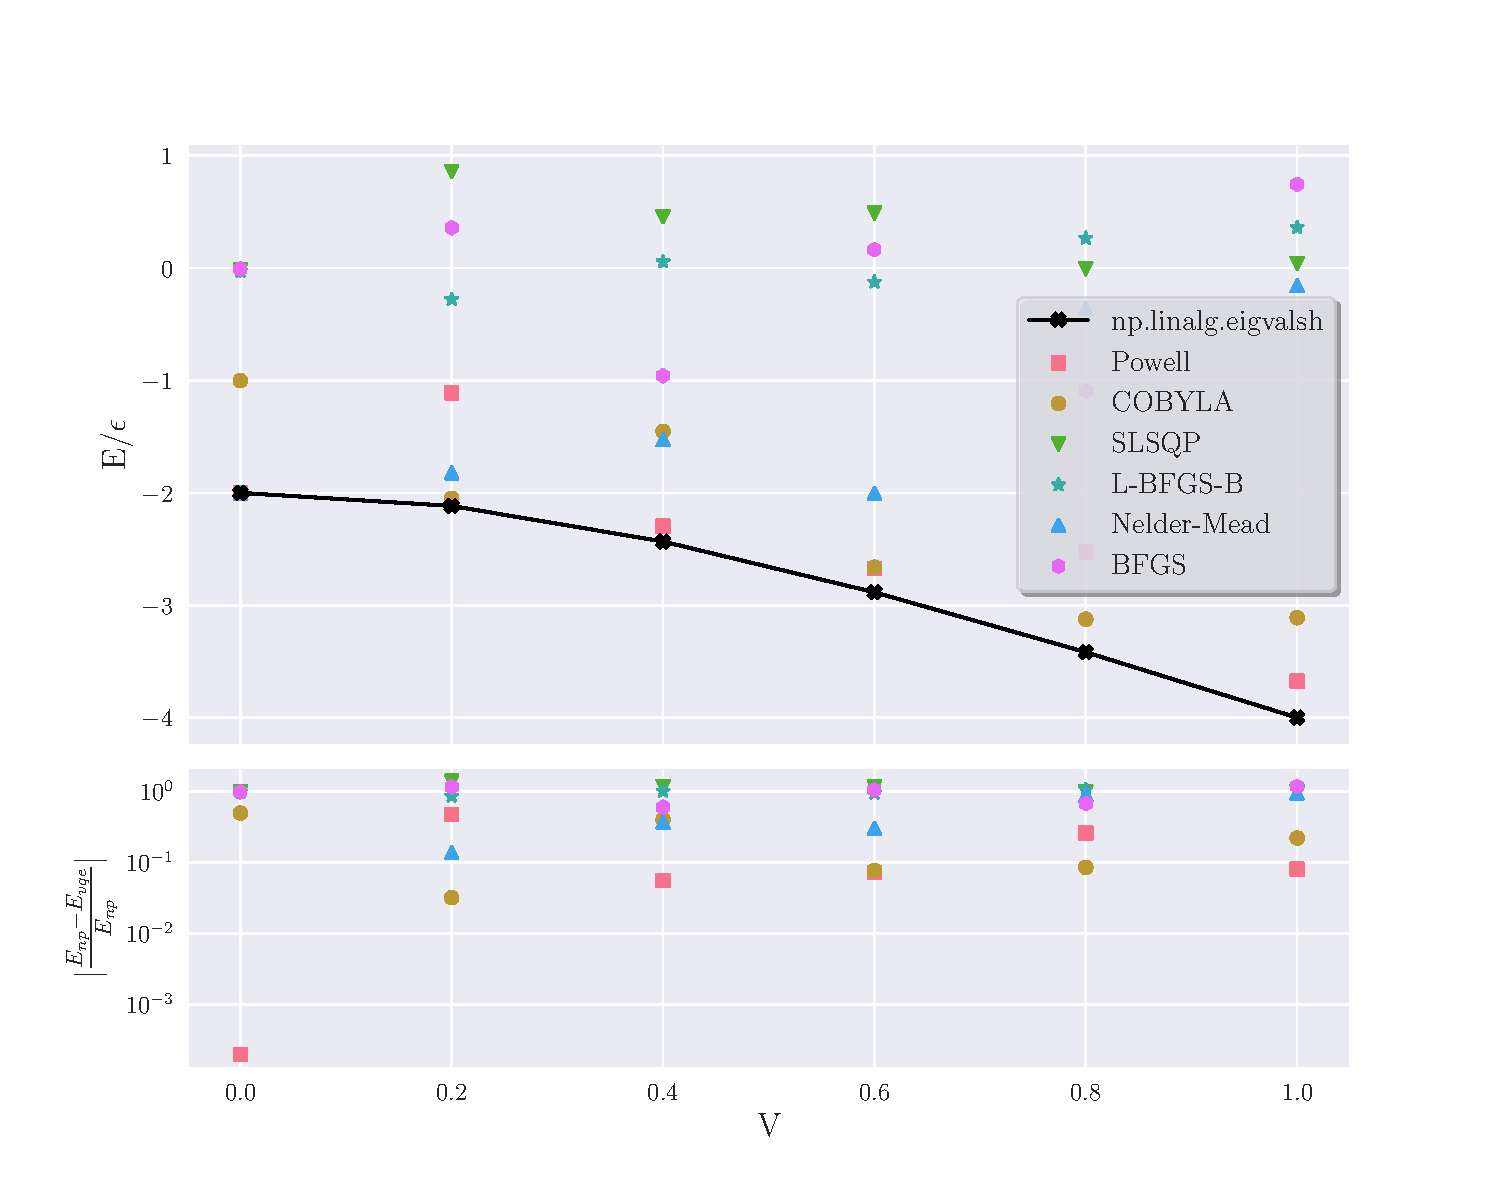
\includegraphics[width=0.32\linewidth]{image/lipkin_result/vqe-opt/cmp_opt_vqe_ee100000_J=2.pdf}
	\caption{Comparison amongst different optimisers for the fixed-form ansatz with \textbf{ideal simulation} for $ J=2 $.}
	\label{fig:OptHW2}
\end{figure}

\begin{figure}[ht]
    \centering
    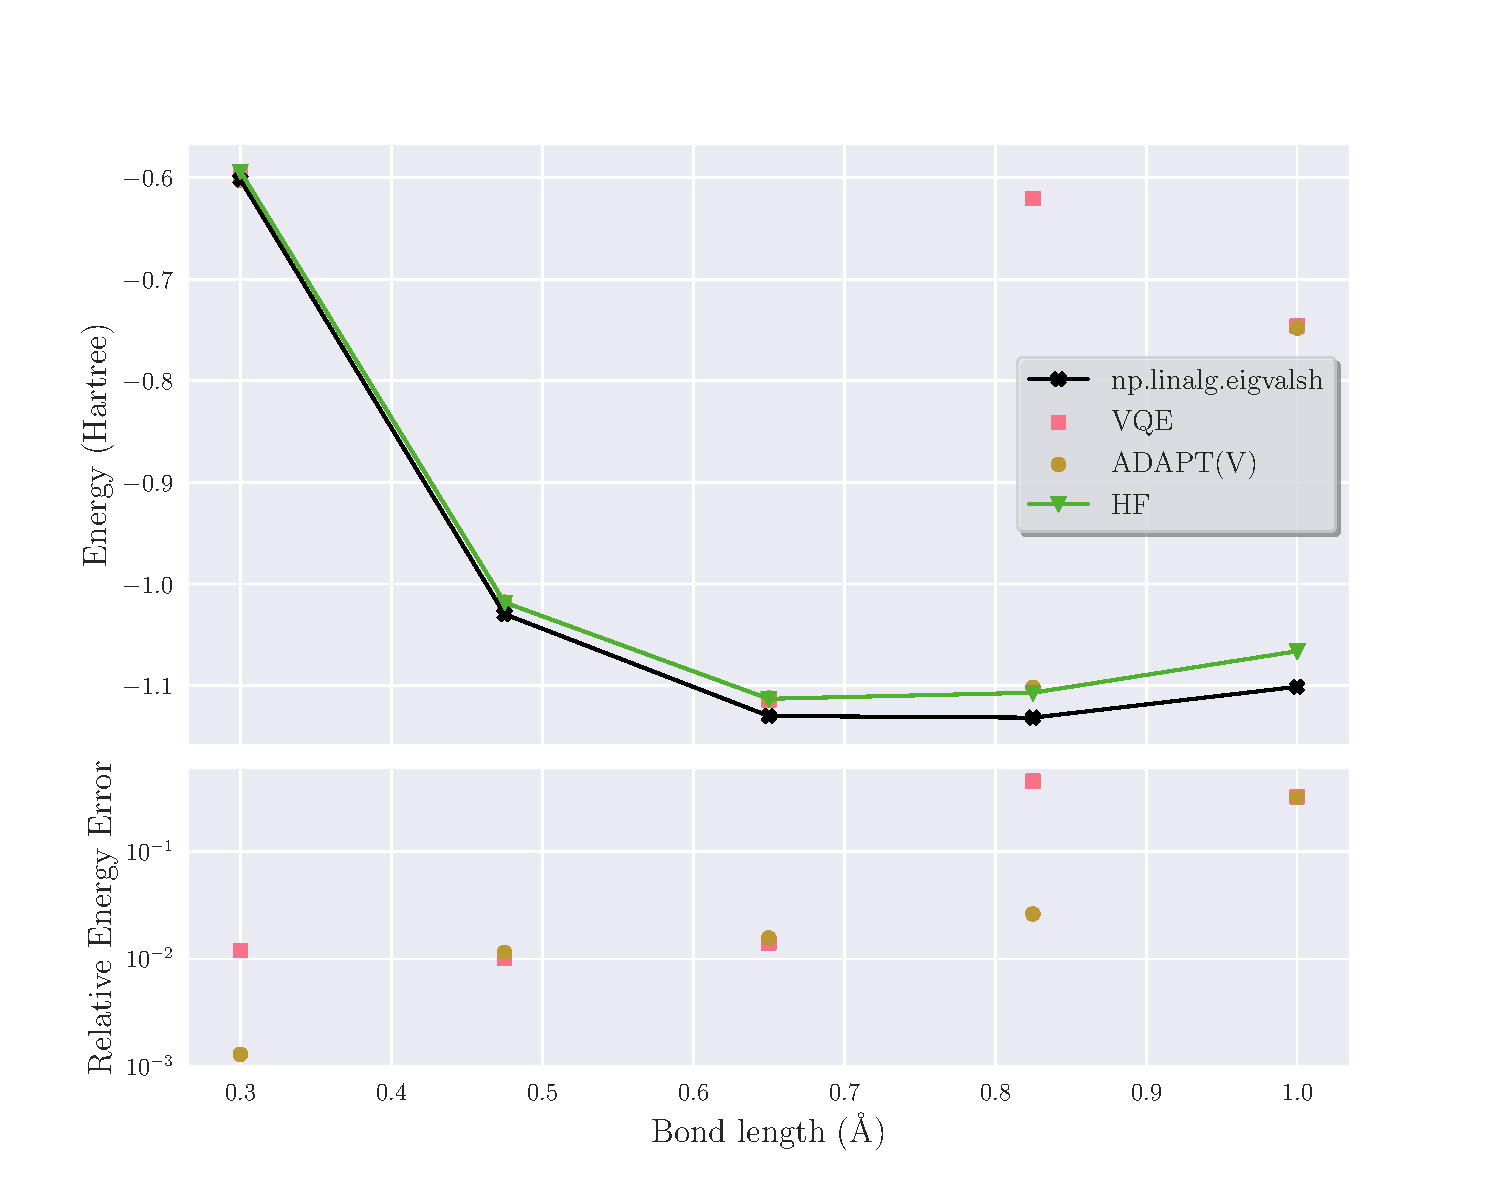
\includegraphics[width=0.47\linewidth]{image/h2_result/simulation/60iter.pdf}
    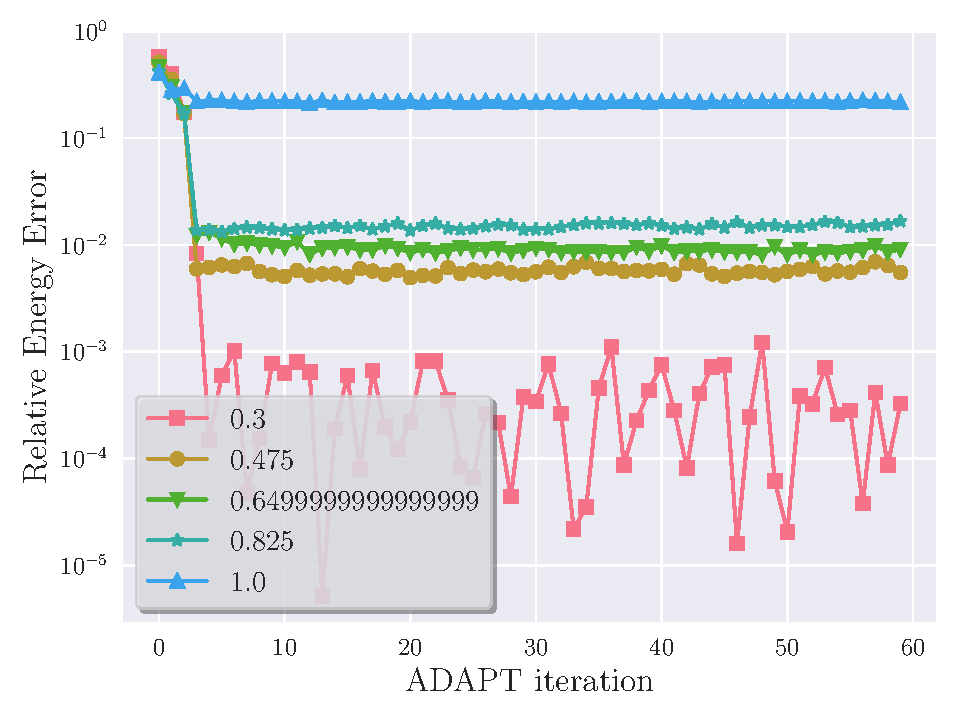
\includegraphics[width=0.45\linewidth]{image/h2_result/simulation/60iter_adapt_err.pdf}
    \caption{(Left) The hydrogen molecule with \textbf{ideal simulation} with $ 100000 $ shots for a maximum of $ 60 $ ADAPT iterations. The ADAPT-VQEs were optimised with the \texttt{COBYLA} method and the VQE with the \texttt{Powell} method. The exponential was decomposed using the \textbf{inverted Staircase} algorithm. (Right) The error at every ADAPT iteration.}
    \label{fig:60iterh2}
\end{figure}



\begin{figure}[ht]
\centering
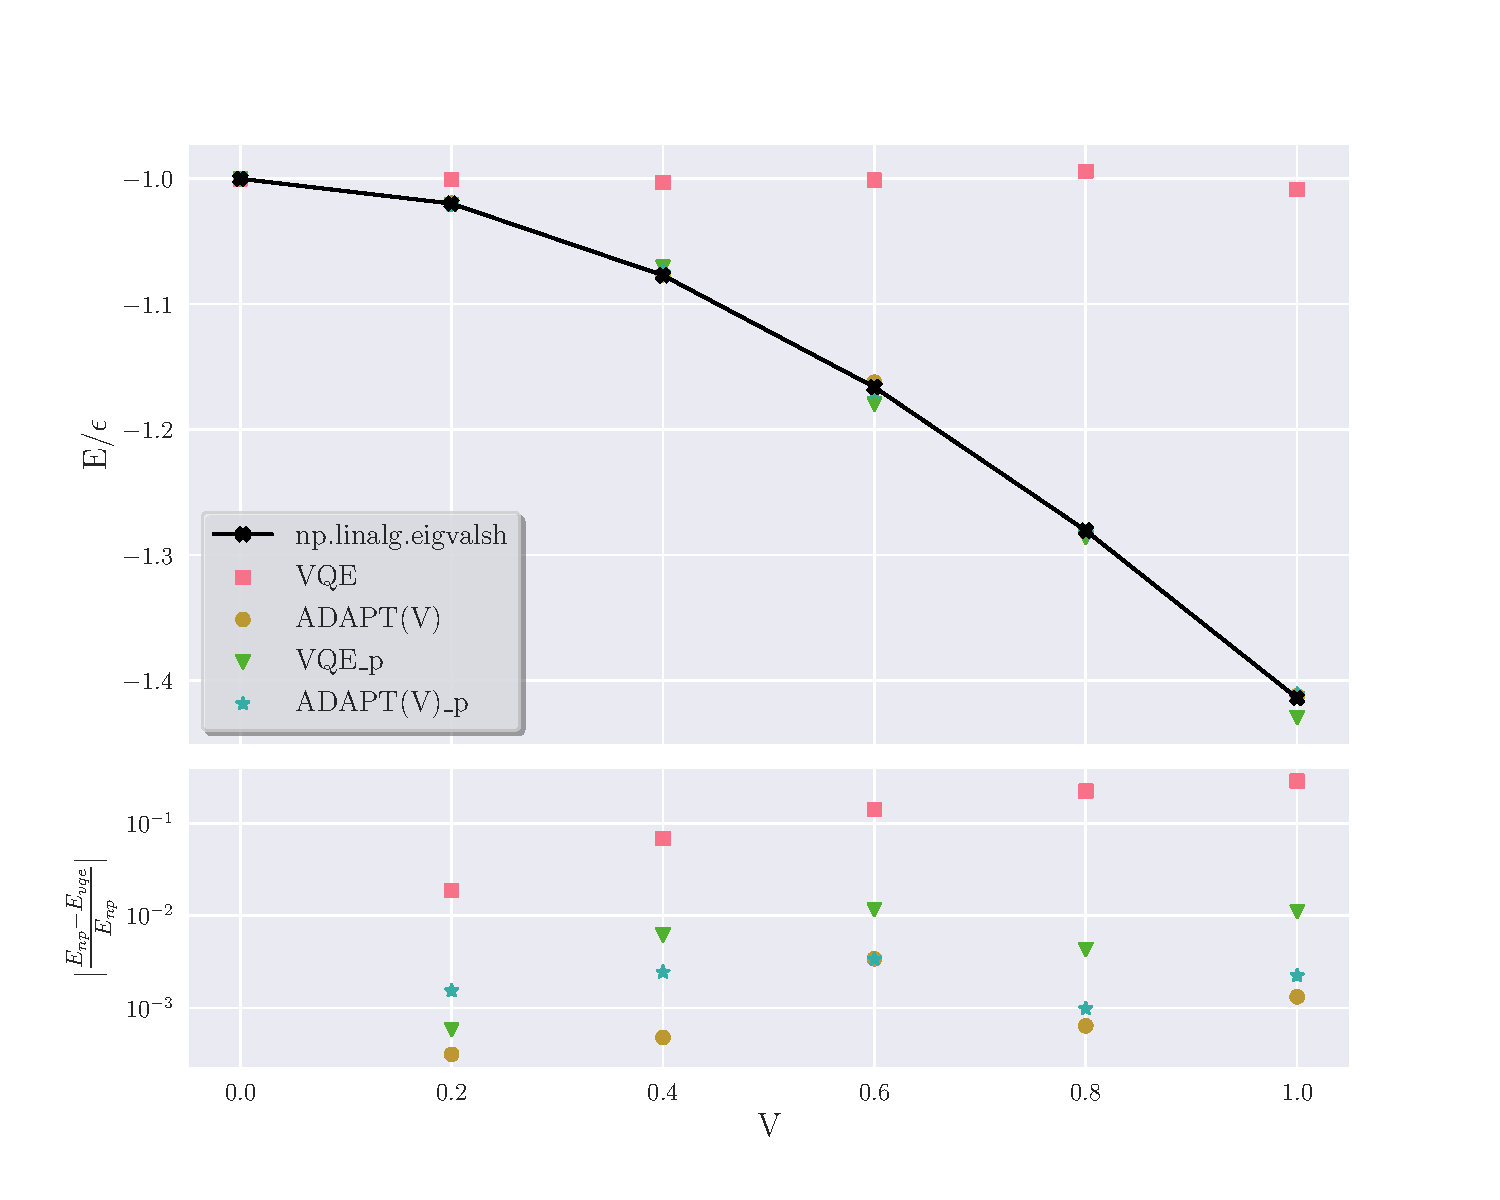
\includegraphics[width=\linewidth]{image/lipkin_result/2repnotok.pdf}
\caption{The LMG model with $ J=1 $ with \textbf{ideal simulation}, showing comparison between VQE with $ 2 $ rep and ADAPT-VQE with the V pool with the V pool and maximum $ 12 $ ADAPT iterations. The ADAPT-VQE was optimised with the \texttt{COBYLA} method and the normal VQE was with \texttt{Powell}. }
\label{fig:2repnotok}
\end{figure}


